\newpage
\section{Hardware Test}

\subsection{Ultraschallsensor}
Als Ultraschallsensor hat man den Typ HC-SR04 getestet. Dieser hat eine Reichweite von 2 cm bis 300 cm mit einer Genauigkeit von 3 mm. Der Sensor wird an 5 V angeschlossen. Mit dem Trigger Pin aktiviert sich die Messung. Der Echo Pin empfängt dabei das, vom Trigger ausgelöste, Signal. Dieser Zeitunterschied zwischen Senden und Empfangen ist dann mit der Schallgeschwindigkeit umgerechnet die Distanz. Die Präzision des Sensors wird mit dem Messaufbau Abbildung \ref{fig:Ultraschall1} ermittelt.

\begin{figure}[h] % 'h' steht für here, was bedeutet, dass das Bild möglichst an dieser Stelle eingefügt wird
    \centering
    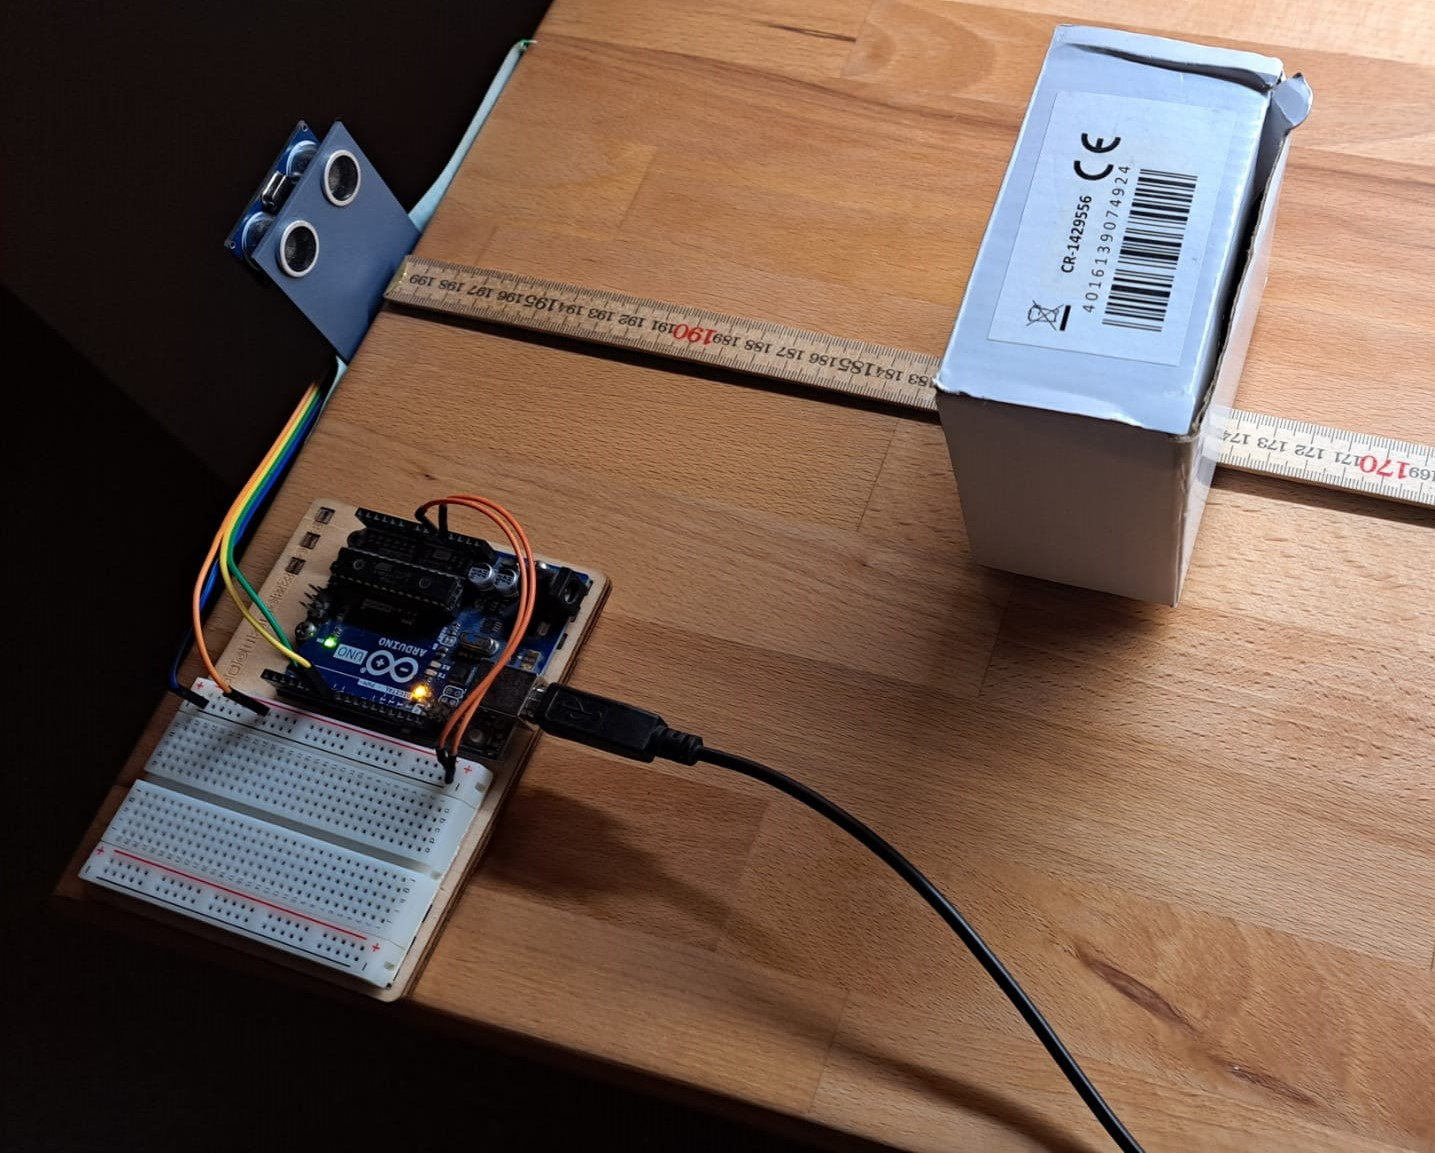
\includegraphics[width=0.5\textwidth]{img/sensortest/MA_Ultraschall.jpg} % Bildname und Breite der Grafik angeben
    \caption{Messaufbau Ultraschallsensor}
    \label{fig:Ultraschall1} % Label für die Referenzierung der Abbildung
\end{figure}

In diesem Aufbau wird das Objekt je um ein Zentimeter verschoben und den dazugehörenden Messwert aufgeschrieben. Daraus ergaben sich folgende Messwerte:
\begin{table}[H]
\centering
\begin{minipage}{0.45\textwidth}
\centering
\begin{tabular}{@{}ll@{}}
\toprule
\textbf{Position} & \textbf{Messwert} \\
\midrule
10 mm  & 22 mm  \\
20 mm  & 25 mm  \\
30 mm  & 31 mm  \\
40 mm  & 41 mm  \\
50 mm  & 54 mm  \\
60 mm  & 61 mm  \\
70 mm  & 69 mm  \\
80 mm  & 82 mm  \\
90 mm  & 89 mm  \\
100 mm & 95 mm  \\
\bottomrule
\end{tabular}
\end{minipage}%
\hspace{0.05\textwidth} % kleiner Abstand zwischen den Tabellen
\begin{minipage}{0.45\textwidth}
\centering
\begin{tabular}{@{}ll@{}}
\toprule
\textbf{Position} & \textbf{Messwert} \\
\midrule
110 mm & 112 mm \\
120 mm & 121 mm \\
130 mm & 130 mm \\
140 mm & 136 mm \\
150 mm & 149 mm \\
160 mm & 160 mm \\
170 mm & 170 mm \\
180 mm & 181 mm \\
190 mm & 190 mm \\
200 mm & 205 mm \\
\bottomrule
\end{tabular}
\end{minipage}
\caption{Ultraschallsensor Messwerte}
\label{tab:UltraschallMD}
\end{table}

Aus der Tabelle \ref{tab:UltraschallMD} fällt auf, dass die Messdaten ganz in der Nähe des Sensors ungenauer sind. Entfernt sich das Objekt, wird er präziser. Das bedeutet bei der Wahl des Ultraschallsensors muss der Einbauort mindestens 3 cm vom Hindernis entfernt sein. 

\newpage
\subsection{Time of Flight Sensor}
Ein Time of Flight Sensor (TOF) funktioniert ähnlich wie der Ultraschallsensor. Ausser, dass ein Lichtstrahl anstatt von einer Schallwelle ausgesendet wird. In diesem Versuch wird der TOF Typ VL530LX getestet. Der Messaufbau ist derselbe wie bei dem Ultraschallsensor (siehe Abbildung \ref{fig:TOF1}).

\begin{figure}[h!] % 'h' steht für here, was bedeutet, dass das Bild möglichst an dieser Stelle eingefügt wird
    \centering
    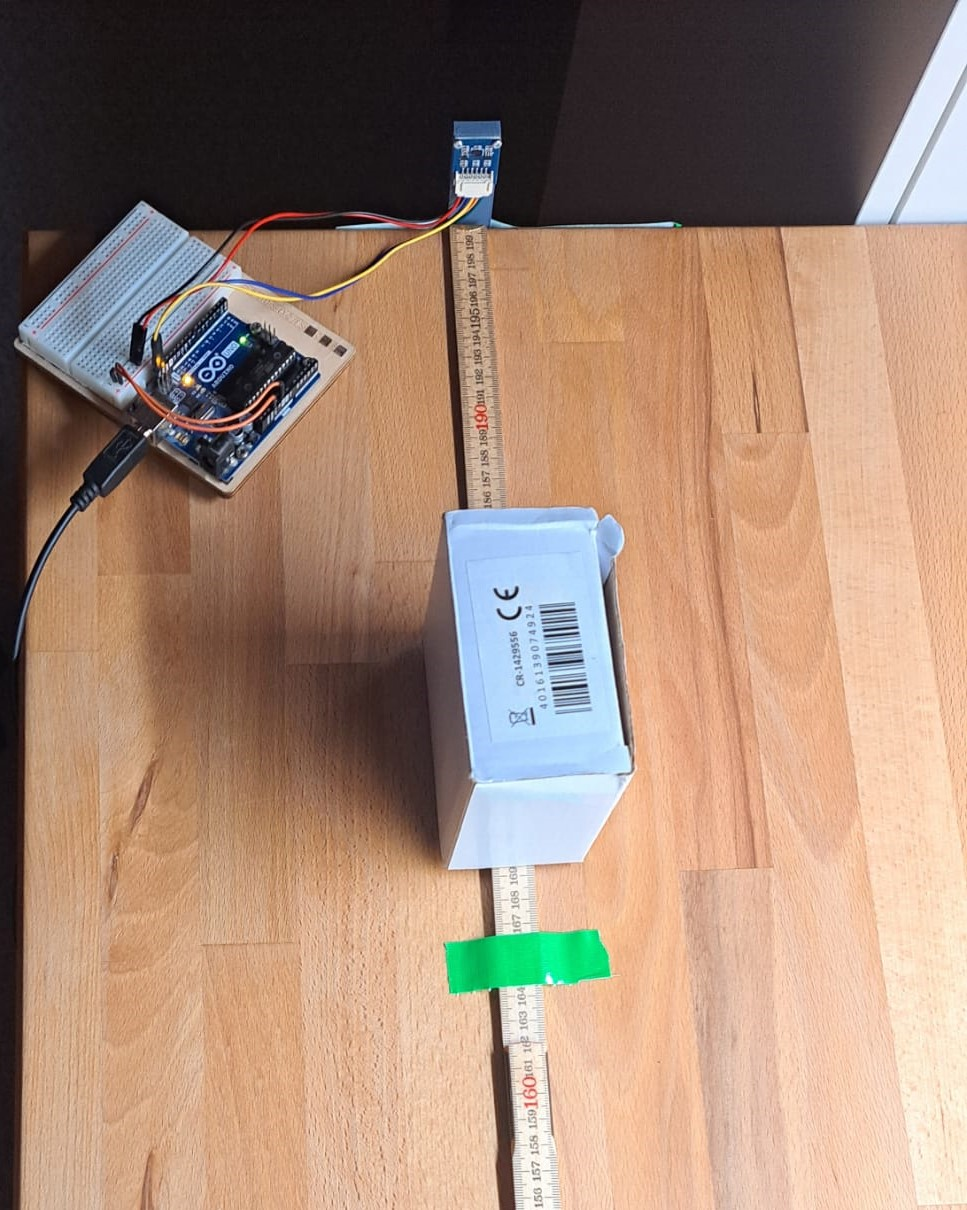
\includegraphics[width=0.35\textwidth]{img/sensortest/MA_TOF.jpg} % Bildname und Breite der Grafik angeben
    \caption{Testaufbau TOF Sensor}
    \label{fig:TOF1} % Label für die Referenzierung der Abbildung
\end{figure}


Auch hier wird das Objekt Zentimeter für Zentimeter nach vorne bewegt und die Messdaten notiert. Dabei ergaben sich folgende Messwerte:
\begin{table}[H]
\centering
\begin{minipage}{0.45\textwidth}
\centering
\begin{tabular}{@{}ll@{}}
\toprule
\textbf{Position} & \textbf{Messwert} \\
\midrule
10 mm  & 11 mm  \\
20 mm  & 24 mm  \\
30 mm  & 31 mm  \\
40 mm  & 43 mm  \\
50 mm  & 51 mm  \\
60 mm  & 63 mm  \\
70 mm  & 72 mm  \\
80 mm  & 84 mm  \\
90 mm  & 93 mm  \\
100 mm & 102 mm \\
\bottomrule
\end{tabular}
\end{minipage}%
\hspace{0.05\textwidth} % kleiner Abstand zwischen den Tabellen
\begin{minipage}{0.45\textwidth}
\centering
\begin{tabular}{@{}ll@{}}
\toprule
\textbf{Position} & \textbf{Messwert} \\
\midrule
110 mm & 115 mm \\
120 mm & 125 mm \\
130 mm & 132 mm \\
140 mm & 145 mm \\
150 mm & 151 mm \\
160 mm & 163 mm \\
170 mm & 170 mm \\
180 mm & 182 mm \\
190 mm & 190 mm \\
200 mm & 200 mm \\
\bottomrule
\end{tabular}
\end{minipage}
\caption{TOF Messwerte}
\label{tab:TOFMD}
\end{table}

Aus der Tabelle \ref{tab:TOFMD} erkennt man, dass der Messwert in der Nähe des Sensors relativ präzise ist. Ebenso scheint der Sensor auch genau in die Ferne zu sein. Diese Messungen machen den TOF Sensor zu der bevorzugten Distanzmessart für das Hindernis.


\subsection{Farbsensor}
Der Farbsensor, welcher hier getestet wird, hat die Typenbezeichnung TCS34725. Dieser kommuniziert über eine I2C Schnittstelle und liefert folgende Werte: Rotwert, Grünwert, Blauwert und der Clearwert. Ebenso kann der Temperaturwert und der Lux Wert aus diesen berechnet werden. In diesem Testversuchgeht es darum, den Wert zu identifizieren, welcher auf den verschieden Bodenbeschaffenheiten den grössten Unterschied aufzeigt. Damit die Messungen reproduzierbar sind, wurde ein Halter gedruckt, welcher den Sensor 1 cm über dem Boden hält (siehe Abbildung \ref{fig:Farbsensorhalter}).


\begin{figure}[H] % 'h' steht für here, was bedeutet, dass das Bild möglichst an dieser Stelle eingefügt wird
    \centering
    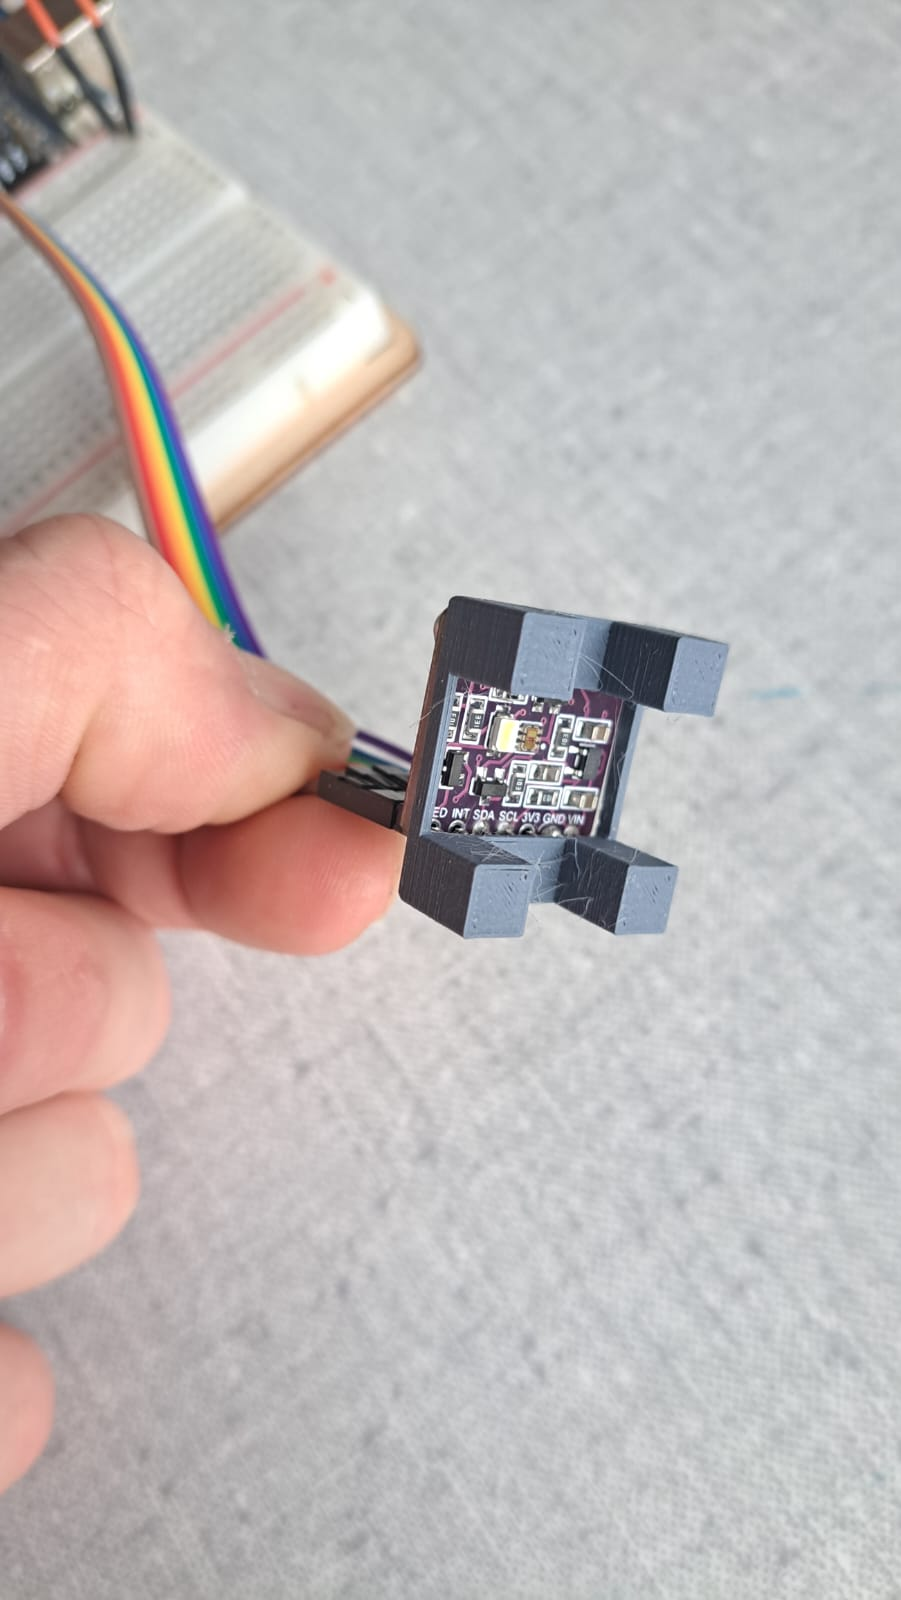
\includegraphics[width=0.2\textwidth]{img/sensortest/FarbsensorHalter.jpg} % Bildname und Breite der Grafik angeben
    \caption{Farbsensorhalter}
    \label{fig:Farbsensorhalter} % Label für die Referenzierung der Abbildung
\end{figure}

Nun werden alle vier möglichen Szenarien getestet, siehe Abbildung \ref{fig:Testanordnungen}. Einmal die Linie, der weisse Punkt, die rote Platte und noch die Fuge. Dabei ist die LED immer eingeschaltet.

\begin{figure}[H]
    \centering
    % Oben links
    \begin{subfigure}{0.3\textwidth} % Breite auf 45% gesetzt, um Platz für zwei Bilder pro Zeile zu schaffen
        \centering
        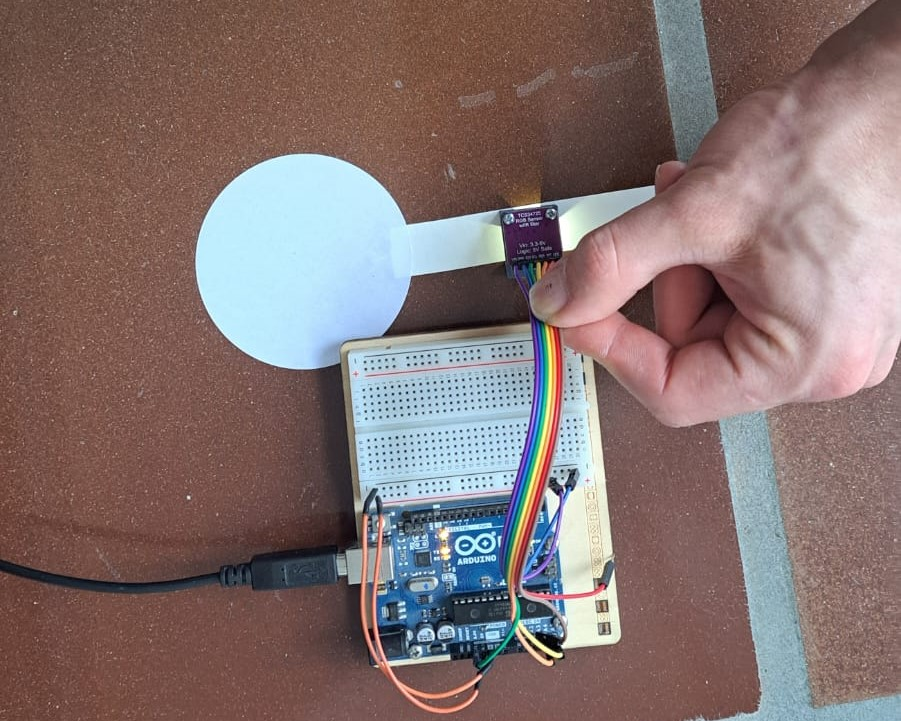
\includegraphics[width=\linewidth]{img/sensortest/Farbsensor_Linie.jpg}
        \caption{Farbsensor Linie}
        \label{fig:FarbsensorLinie}
    \end{subfigure}
    % Oben rechts
    \begin{subfigure}{0.3\textwidth}
        \centering
        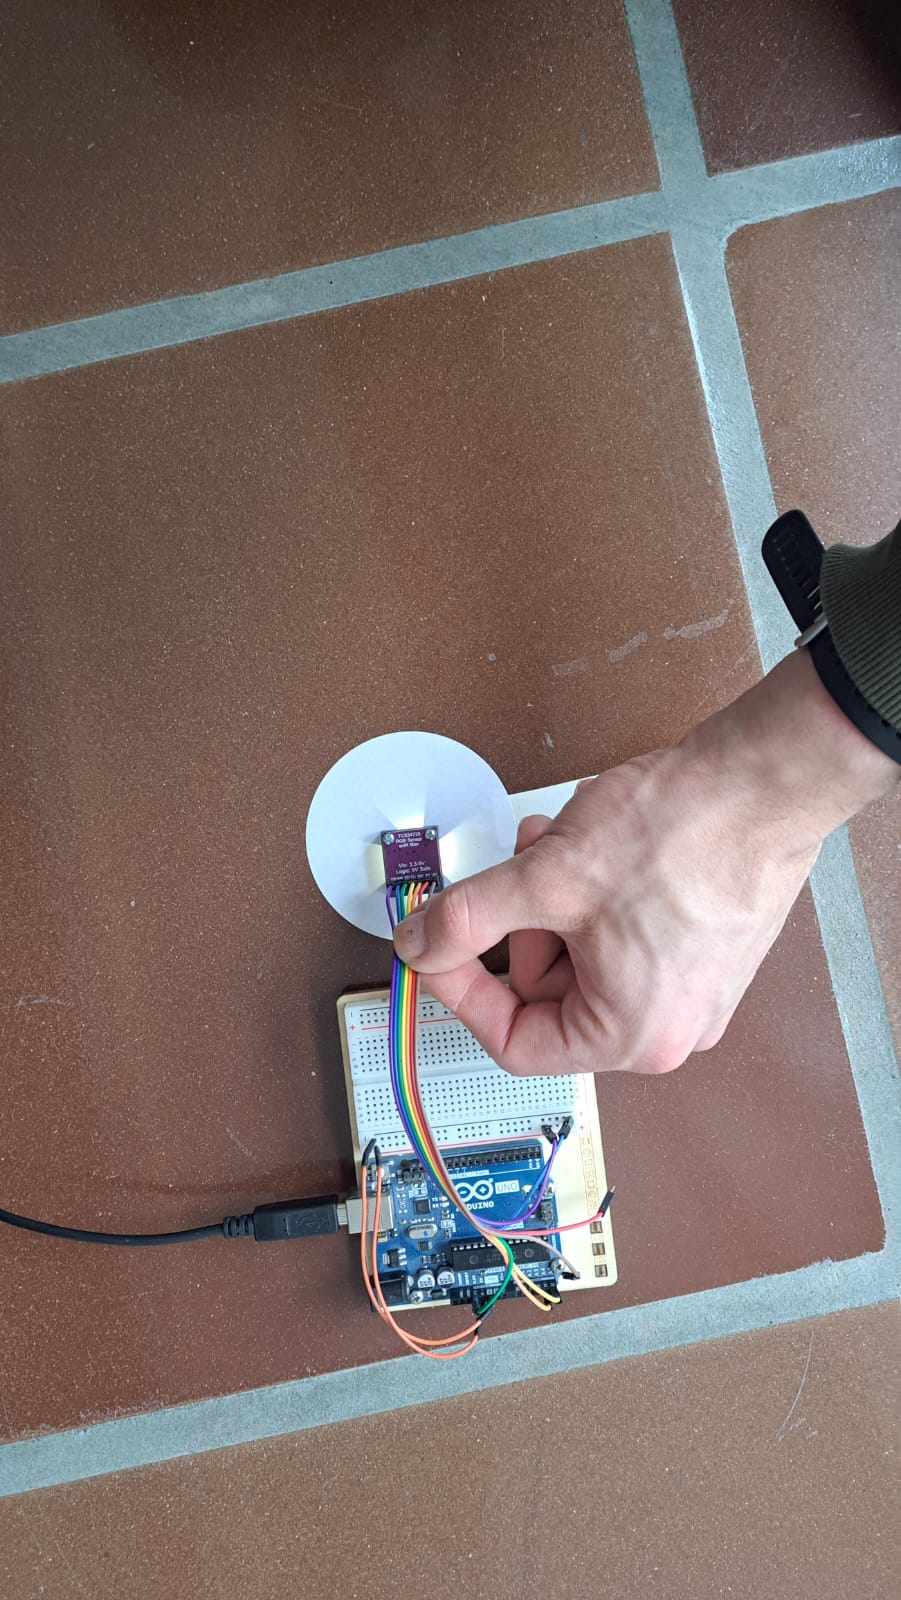
\includegraphics[width=\linewidth]{img/sensortest/Farbsensor_WeisserPunkt.jpg}
        \caption{Farbsensor weisser Punkt}
        \label{fig:FarbsensorWeisserPunkt}
    \end{subfigure}
    
    % Abstand zwischen den Reihen
    \vspace{0.5cm}

    % Unten links
    \begin{subfigure}{0.3\textwidth}
        \centering
        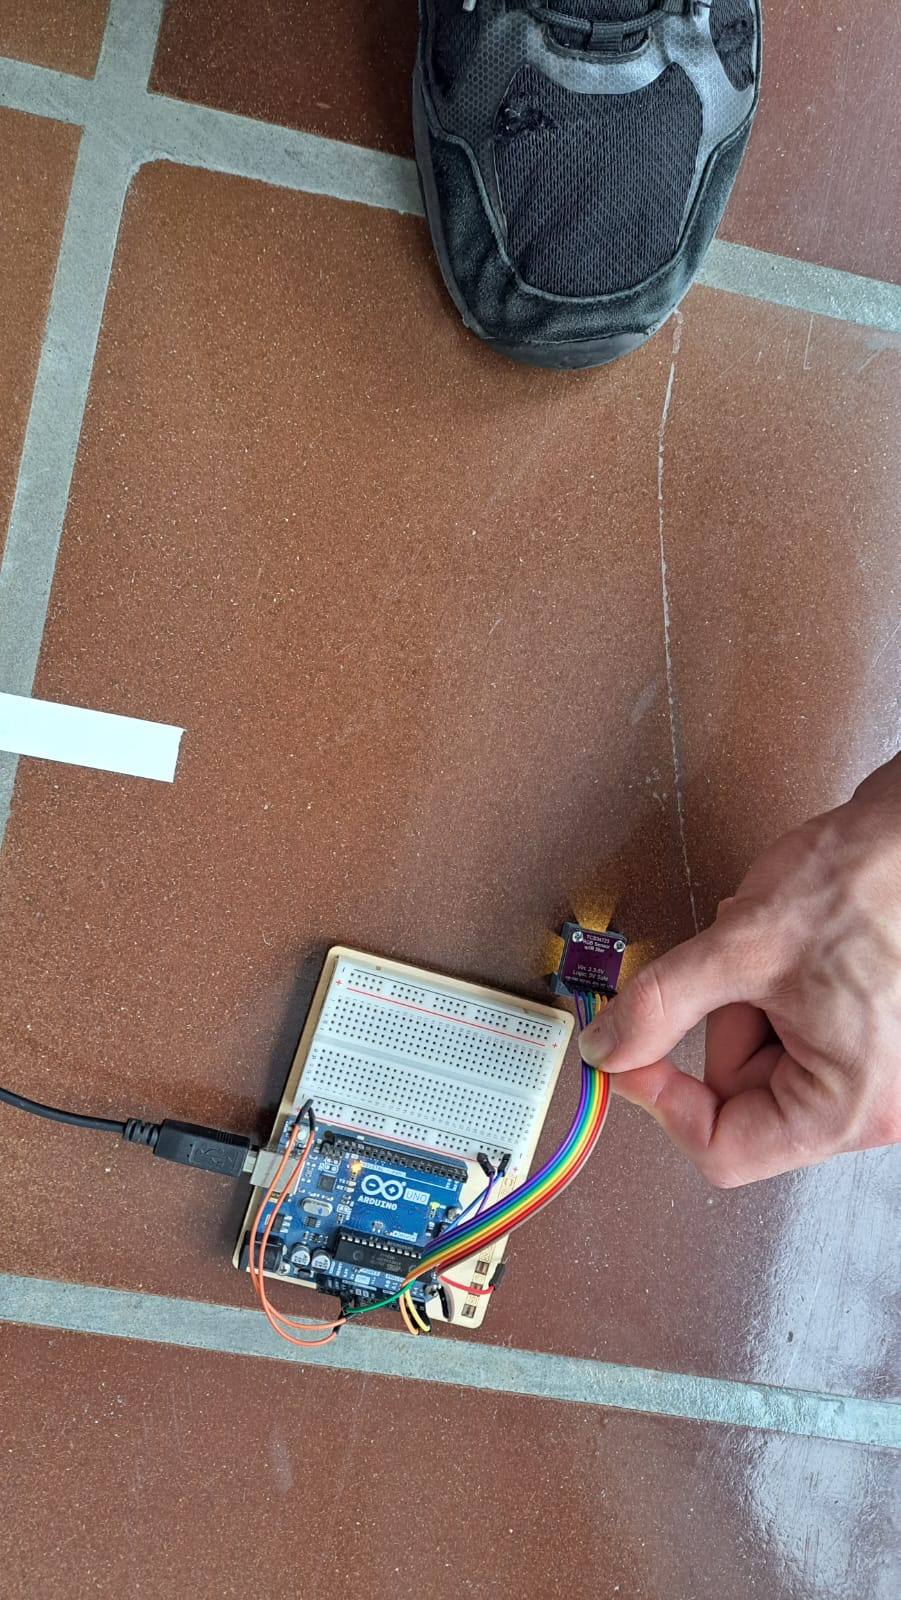
\includegraphics[width=\linewidth]{img/sensortest/Farbsensor_Platte.jpg}
        \caption{Farbsensor Platte}
        \label{fig:FarbsensorPlatte}
    \end{subfigure}
    % Unten rechts
    \begin{subfigure}{0.3\textwidth}
        \centering
        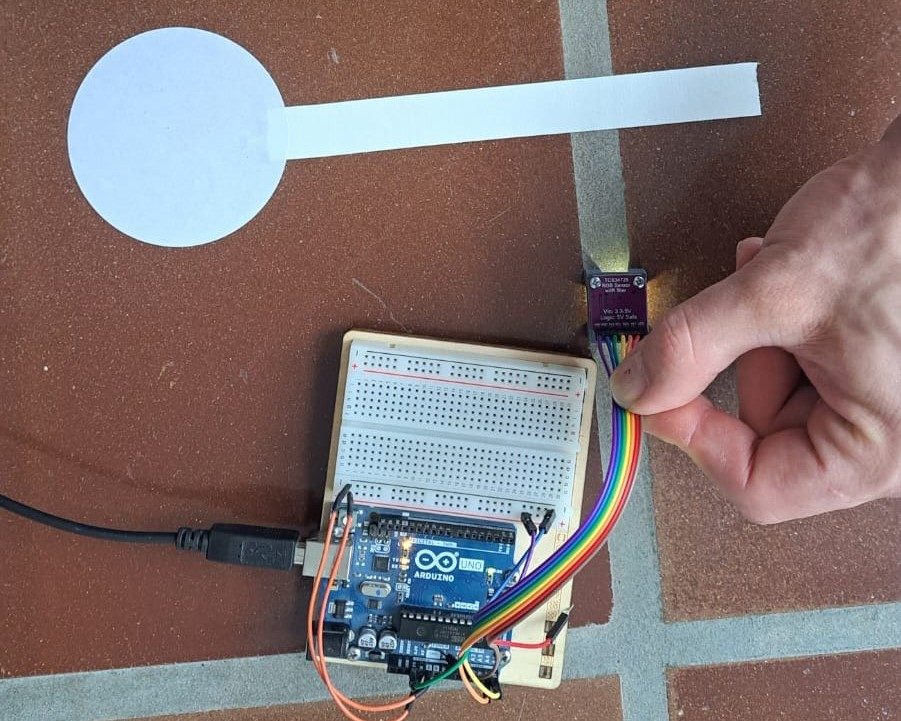
\includegraphics[width=\linewidth]{img/sensortest/Farbsensor_Fuge.jpg}
        \caption{Farbsensor Fuge}
        \label{fig:FarbsensorFuge}
    \end{subfigure}

    \caption{Testaufbau}
    \label{fig:Testanordnungen}
\end{figure}



Das ergab folgende Messdaten:


\begin{figure}[H]
    \centering
    % Oben links
    \begin{subfigure}{0.35\textwidth} % Breite auf 45% gesetzt, um Platz für zwei Bilder pro Zeile zu schaffen
        \centering
        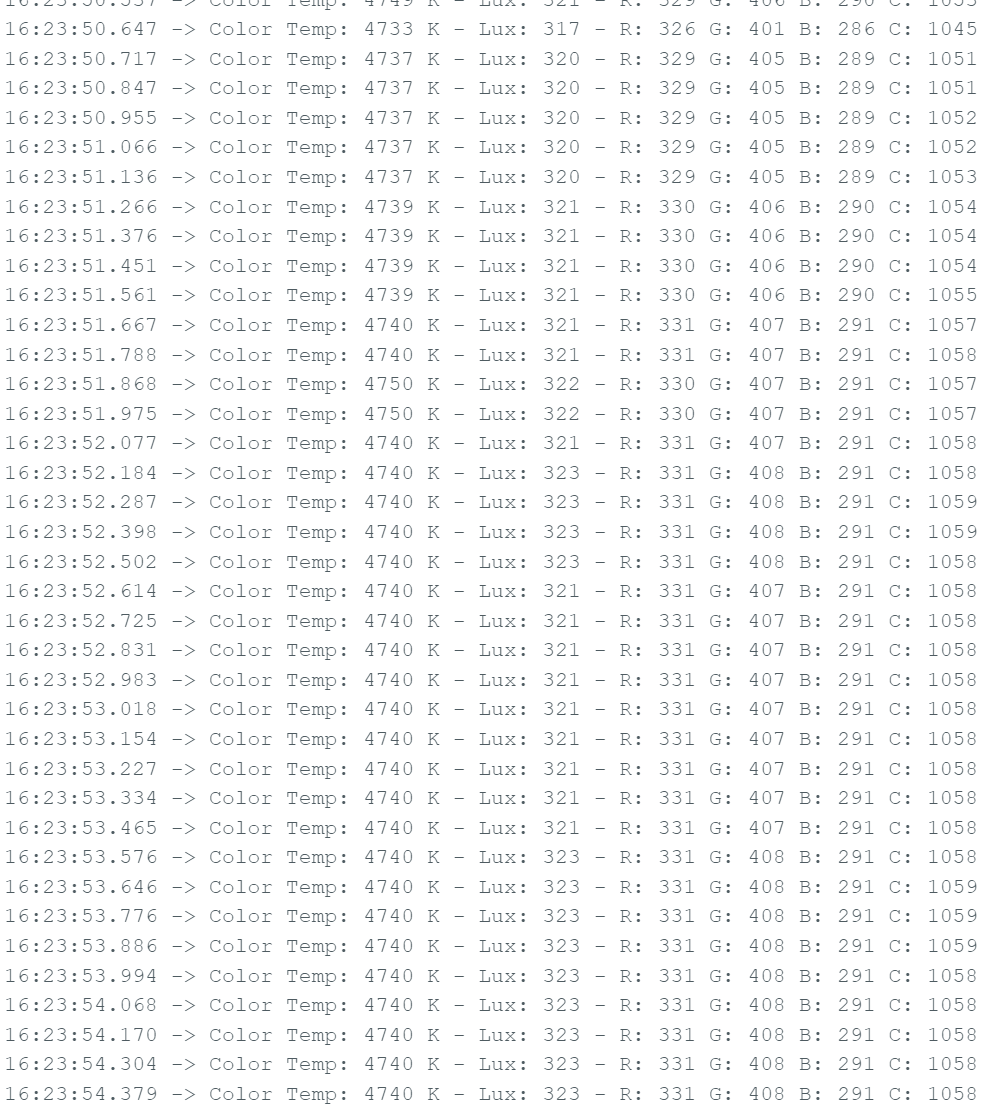
\includegraphics[width=\linewidth]{img/sensortest/MD_Linie_101ms.png}
        \caption{Messdaten Linie}
        \label{fig:MD_Farbsens}
    \end{subfigure}
    % Oben rechts
    \begin{subfigure}{0.35\textwidth}
        \centering
        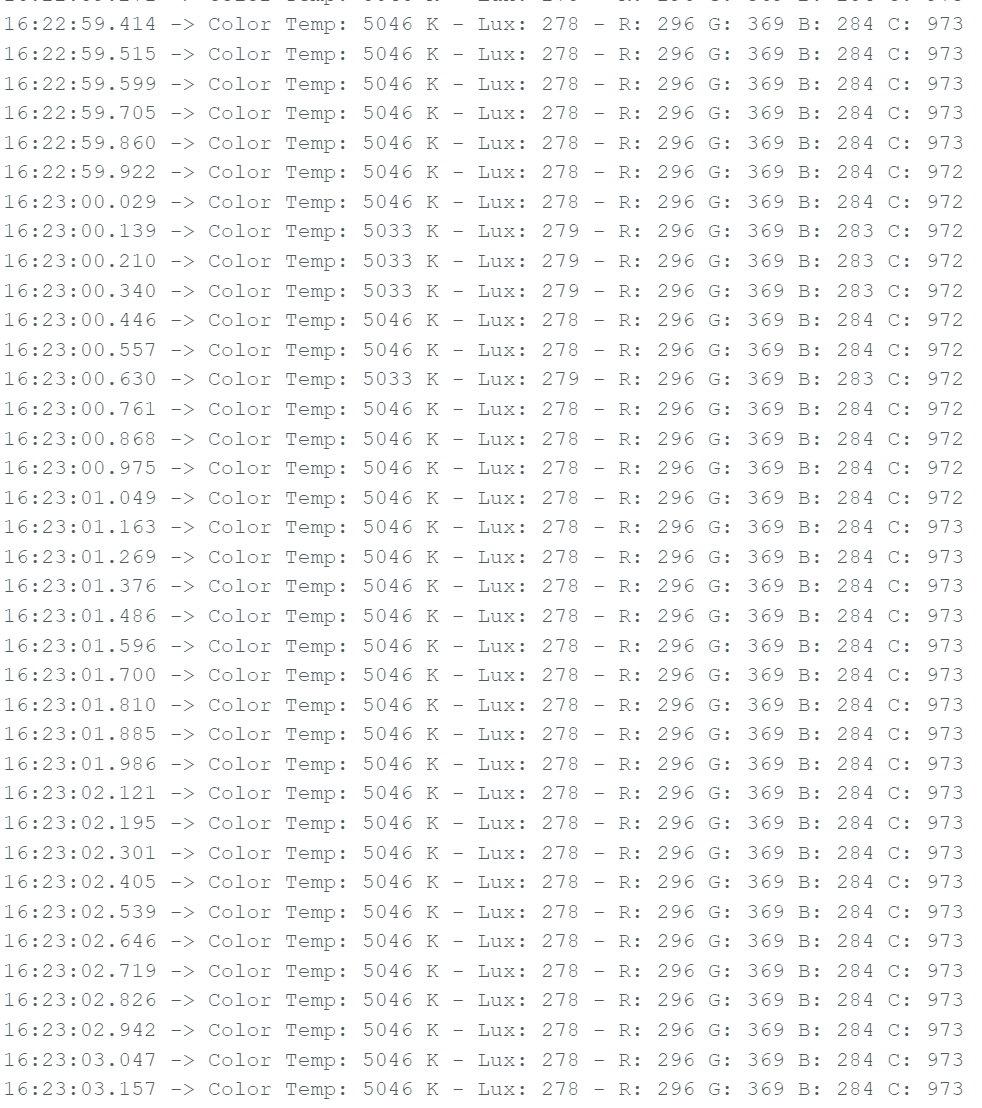
\includegraphics[width=\linewidth]{img/sensortest/MD_WeisserPunkt_101ms.png}
        \caption{Messdaten weisser Punkt}
        \label{fig:MDFarbsensorWeisserPunkt}
    \end{subfigure}
    
    % Abstand zwischen den Reihen
    \vspace{0.5cm}

    % Unten links
    \begin{subfigure}{0.35\textwidth}
        \centering
        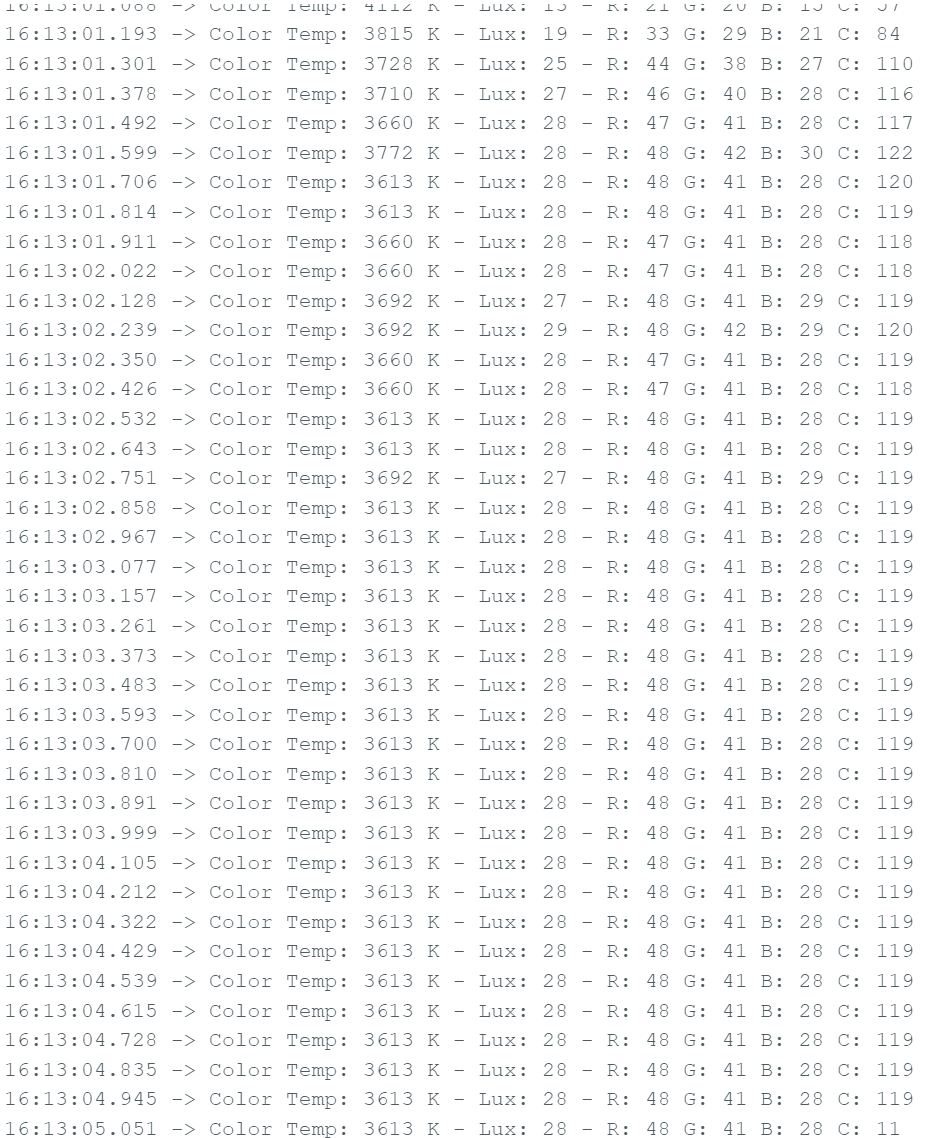
\includegraphics[width=\linewidth]{img/sensortest/MD_RotePlatte_101ms.png}
        \caption{Messdaten rote Platte}
        \label{fig:MDFarbsensorPlatte}
    \end{subfigure}
    % Unten rechts
    \begin{subfigure}{0.35\textwidth}
        \centering
        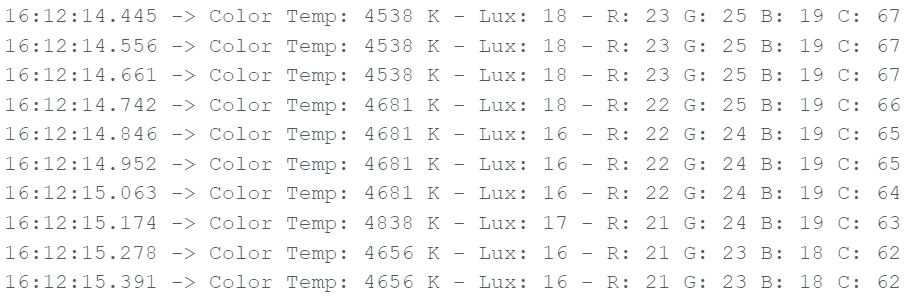
\includegraphics[width=\linewidth]{img/sensortest/MD_Fuge_101ms.png}
        \caption{Messdaten Fuge}
        \label{fig:MDFarbsensorFuge}
    \end{subfigure}

    \caption{Messdaten Farbsensor}
    \label{fig:Testanordnungen}
\end{figure}

Aus den Messdaten geht hervor das der Lux Wert sich am meisten unterscheidet. Dieser hat ein Wert auf der Linie von 320 und auf dem weissen Punkt 280. Somit kann man den Punkt von der Linie unterscheiden. Die rote Platte hat einen Wert von 28 und die Fuge von 14. Diese Werte sind deutlich von den 320 entfernt. Somit kann man mit dem Farbsensor der Linie folgen.

